% !TeX program = pdflatex
% Compilar: pdflatex main; bibtex main; pdflatex main; pdflatex main.
% Entregable parcial: introducción, antecedentes, tres tareas y pipeline.
\documentclass[10pt,a4paper,twocolumn]{article}
\usepackage[utf8]{inputenc}
\IfFileExists{lmodern.sty}{\usepackage[T1]{fontenc}\usepackage{lmodern}}{}
\IfFileExists{spanish.ldf}{\usepackage[spanish,es-tabla,es-nodecimaldot]{babel}}{}
\usepackage[margin=1.85cm,columnsep=0.65cm]{geometry}
\usepackage{amsmath,amssymb,booktabs,tabularx,array,enumitem,microtype}
\usepackage{tikz}
\usetikzlibrary{arrows.meta,positioning,calc}
\usepackage{xurl,cite,fancyhdr,titlesec,balance}
\usepackage[hidelinks,unicode]{hyperref}
\hypersetup{pdftitle={Análisis visual y predicción de hotspots delictivos en Chicago con Transformer Hawkes Process},pdfauthor={Alex Maglio Neyra Herrada},pdflang={es}}
\renewcommand{\abstractname}{Resumen}
\renewcommand{\refname}{Referencias}
\renewcommand{\tablename}{Tabla}
\renewcommand{\figurename}{Figura}
\renewcommand{\thesection}{\Roman{section}}
\renewcommand{\thesubsection}{\Alph{subsection}}
\titleformat{\section}{\large\bfseries\raggedright}{\thesection.}{0.6em}{}
\titleformat{\subsection}{\normalsize\bfseries\raggedright}{\thesubsection.}{0.6em}{}
\titlespacing*{\section}{0pt}{1.8ex plus 0.4ex}{0.9ex}
\titlespacing*{\subsection}{0pt}{1.5ex plus 0.3ex}{0.7ex}
\raggedbottom
\newcolumntype{Y}{>{\raggedright\arraybackslash}X}
\newcommand{\campo}[1]{\texttt{#1}}
\newcommand{\tarea}[1]{\textbf{T#1}}
\setlength{\parindent}{1em}
\setlength{\parskip}{0.15em}
\setlength{\emergencystretch}{1.7em}
\setlist[itemize]{leftmargin=*,itemsep=2pt,topsep=4pt}
\definecolor{azul}{HTML}{234B66}
\definecolor{fondo}{HTML}{EDF3F7}
\pagestyle{fancy}
\fancyhf{}
\fancyhead[L]{\footnotesize Neyra Herrada}
\fancyhead[R]{\footnotesize THP y hotspots en Chicago}
\fancyfoot[C]{\thepage}
\setlength{\headheight}{13pt}
\renewcommand{\headrulewidth}{0.3pt}
\renewcommand{\topfraction}{0.92}
\renewcommand{\dbltopfraction}{0.92}
\renewcommand{\textfraction}{0.07}
\renewcommand{\floatpagefraction}{0.8}
\renewcommand{\dblfloatpagefraction}{0.8}

\title{\Large\bfseries Análisis visual y predicción de hotspots delictivos\newline
 en Chicago mediante Transformer Hawkes Process\\[3pt]
\large Propuesta sobre registros de 2001--2026}
\author{Alex Maglio Neyra Herrada\\[2pt]
\small Maestría en Ciencia de la Computación\\
\small Universidad Nacional de San Agustín de Arequipa, Perú\\
\small Curso: Tópicos en Ciencia de Datos}
\date{}

\begin{document}
\twocolumn[\maketitle
\begin{minipage}{\textwidth}
\small
\textbf{Resumen.} Este trabajo propone un sistema de análisis visual y predicción de zonas con mayor concentración futura de delitos registrados en Chicago. El notebook exploratorio disponible contiene 8\,636\,476 registros entre el 1 de enero de 2001 y el 3 de septiembre de 2026. Cada incidente elegible se representará por su tiempo y una marca conjunta de categoría delictiva y distrito policial. Un Transformer Hawkes Process (THP) modelará la intensidad condicional de las marcas; simulaciones condicionadas al historial anterior a cada fecha de pronóstico producirán conteos esperados por distrito para un horizonte de 24 horas. CrimAnalyzer orienta la exploración visual y una factorización no negativa de perfiles horarios, reconstruida como pronosticador temporal, servirá de comparación. Se definen exactamente tres tareas analíticas y un pipeline de datos, entrenamiento, pronóstico y evaluación cronológica. Las cifras del notebook describen el insumo; los pronósticos y sus métricas son componentes propuestos, aún sin resultados experimentales.

\medskip
\textbf{Palabras clave:} predicción de hotspots; procesos puntuales temporales; Transformer Hawkes Process; análisis visual; Chicago; NMF.
\end{minipage}\vspace{1.1em}]
\thispagestyle{plain}

\section{Introducción}
\subsection{Contexto y motivación}
Los registros abiertos de seguridad pública permiten examinar la concentración territorial y temporal de delitos reportados. Para analistas municipales, una estimación verificable de dónde podrían concentrarse los próximos incidentes puede orientar la exploración y la planificación. Un mapa de conteos históricos, sin embargo, no determina por sí solo dónde se concentrarán los eventos en una fecha futura. Además, la interpretación depende de la cobertura del registro, de la granularidad espacial y de qué se entiende por incidente.

El portal de Chicago publica el conjunto \emph{Crimes -- 2001 to Present}, procedente de CLEAR y con ubicaciones aproximadas a nivel de cuadra \cite{chicagoCrimes}. El notebook que acompaña al informe exploratorio aprobado \cite{neyra2026informe} conserva una carga de 8\,636\,476 filas y 22 columnas; el mínimo y máximo guardados de \campo{Date} son 2001-01-01 00:00:00 y 2026-09-03 00:00:00. La presente propuesta toma \emph{todo ese intervalo} como alcance de la fuente. El extremo de 2026 corresponde a un año incompleto y las cifras de este párrafo provienen de salidas guardadas, no de un nuevo entrenamiento. En la fuente, los homicidios pueden publicarse por víctima; la unidad de análisis debe hacerse explícita antes de evaluar un pronóstico \cite{chicagoCrimes}.

Computacionalmente, la dificultad es aprovechar el orden de millones de sucesos sin convertir toda la historia en una única secuencia de autoatención. La factorización no negativa (NMF) explorada en el notebook resume frecuencias por zona y hora, pero la agregación elimina intervalos entre incidentes. Un proceso puntual temporal marcado expresa una tasa condicional para el siguiente evento dado el historial observado \cite{rasmussen2018notes}. Transformer Hawkes Process (THP) combina ese formalismo con autoatención causal para secuencias irregulares \cite{zuo2020thp}. Aquí se plantea una adaptación a marcas conjuntas de tipo de delito y distrito, con una ruta de cómputo acotada y evaluación retrospectiva.

\subsection{Problema y objetivo}
El problema es \emph{predecir, a partir de incidentes anteriores a una fecha de corte, qué distritos concentrarán más delitos registrados durante un horizonte futuro definido y permitir examinar dónde y cuándo el pronóstico falla}. La pregunta rectora es: \emph{¿en qué medida un THP de eventos marcados por delito y distrito identifica los hotspots de las próximas 24 horas frente a un pronóstico basado en NMF, y cómo pueden compararse visualmente las predicciones con las observaciones posteriores?}

El objetivo es diseñar y evaluar un sistema reproducible que (i) represente incidentes como eventos en tiempo continuo; (ii) estime conteos futuros por distrito mediante THP; y (iii) conecte mapas, series temporales y comparación de errores con tres tareas analíticas. La contribución propuesta es la integración y validación de esta formulación en Chicago, inspirada en la exploración de CrimAnalyzer \cite{garcia2021crimanalyzer}; no se afirma haber inventado THP ni demostrado superioridad empírica. Un hotspot indicará \emph{más incidentes registrados esperados}, no riesgo individual, causalidad ni necesidad policial automática: la exposición poblacional no forma parte del modelo.

\section{Trabajos relacionados}
\subsection{Modelos de eventos y características}
Los procesos puntuales describen incidentes mediante tiempos de ocurrencia e intensidad condicionada al pasado \cite{rasmussen2018notes}. Mohler et al. aplicaron un proceso puntual autoexcitante a delitos, antecedente directo para pasar de concentración histórica a predicción de ocurrencias \cite{mohler2011crime}. THP, de Zuo et al., sustituye estados recurrentes de modelos neuronales de procesos puntuales por autoatención y codificación temporal; también contempla relaciones estructurales entre procesos \cite{zuo2020thp}. Su trabajo motiva el modelo temporal, pero este proyecto debe comprobar la adaptación conjunta delito--distrito y su rendimiento en Chicago: esa codificación espacial categórica no equivale a inventar un modelo geográfico continuo.

EasyTPP reúne implementaciones y protocolos de entrenamiento y evaluación de procesos puntuales, incluido THP, y facilita reutilizar el cálculo de verosimilitud y el muestreo \cite{xue2024easytpp}. Se propone usar su implementación PyTorch y documentar el commit y la configuración empleados. La preparación de marcas, la comprobación de máscaras de pérdida y la traducción de intensidades a mapas de horizonte futuro siguen siendo trabajo específico de esta propuesta.

CrimAnalyzer estudia patrones de criminalidad en São Paulo mediante NMF dispersa, umbralización y vistas coordinadas \cite{garcia2021crimanalyzer}. NMF construye componentes aditivos para matrices no negativas \cite{lee1999nmf}. En el notebook de Chicago ya existe una NMF descriptiva de área comunitaria por hora con cuatro factores. Para medir capacidad predictiva se necesita reconstruirla con entrenamiento cronológico, distritos y una regla de extrapolación conocida antes de observar el día evaluado; su factorización descriptiva actual no es un pronóstico comparable. Luo et al. extraen características de series multivariadas ambientales mediante aprendizaje autosupervisado y visualización \cite{luo2024airquality}; su objetivo difiere de estimar tiempos y marcas de incidentes, pero muestra otra vía de representación temporal.

\subsection{Visualización analítica y evaluación espacial}
CrimAnalyzer vincula patrones extraídos con la exploración de regiones y tiempos \cite{garcia2021crimanalyzer}. Voila sitúa anomalías espacio-temporales dentro de su contexto e incorpora retroalimentación del analista \cite{cao2018voila}. AirLens permite explorar variaciones de calidad del aire a varios niveles mediante agrupación y resúmenes visuales \cite{qu2022airlens}. AQX coordina vistas para inspeccionar factores asociados con pronósticos ambientales y contrastarlos con conocimiento del dominio \cite{velumani2022aqx}. Estos trabajos sustentan la necesidad de vincular mapa, serie y comparación, aunque sus datos y modelos no constituyen pruebas de rendimiento del sistema propuesto.

Chainey et al. evaluaron mapas de hotspots frente a incidentes futuros e introdujeron el índice PAI, que divide la proporción de eventos capturados por la proporción de superficie seleccionada \cite{chainey2008utility}. Esta distinción importa en distritos de áreas desiguales. Se compararán THP y NMF con los mismos territorios, horizontes y presupuestos espaciales; una ganancia visualmente atractiva sin prueba fuera de muestra no bastará para sostener el aporte.

\begin{table*}[t]
\centering
\caption{Antecedentes y función en la propuesta. ``Predicción'' describe el objetivo del trabajo citado y no constituye una evaluación cruzada entre estudios.}
\label{tab:relacionados}
\small
\setlength{\tabcolsep}{4.3pt}
\renewcommand{\arraystretch}{1.13}
\begin{tabularx}{\textwidth}{@{}>{\raggedright\arraybackslash}p{2.5cm}YYYY@{}}
\toprule
\textbf{Trabajo} & \textbf{Datos y propósito} & \textbf{Método} & \textbf{Visualización o salida} & \textbf{Uso en Chicago}\\
\midrule
Mohler et al. \cite{mohler2011crime} & Crimen, ocurrencia futura. & Proceso puntual autoexcitante. & Pronóstico de concentración espacial. & Antecedente de eventos y predicción.\\
\addlinespace
THP \cite{zuo2020thp} y EasyTPP \cite{xue2024easytpp} & Eventos asíncronos, siguiente marca y tiempo. & Autoatención causal, intensidad condicional; biblioteca de entrenamiento. & Predicciones de eventos; vistas a diseñar. & Modelo principal y soporte de implementación.\\
\addlinespace
CrimAnalyzer \cite{garcia2021crimanalyzer} & Crimen en São Paulo, exploración de patrones. & NMF dispersa y umbralización. & Vistas espacio-temporales coordinadas. & Referente visual; NMF reconstruida como comparador.\\
\addlinespace
Voila \cite{cao2018voila} & Flujos espacio-temporales, anomalías. & Descomposición tensorial. & Contexto y monitoreo interactivo. & Orienta inspección contextual de errores.\\
\addlinespace
AirLens \cite{qu2022airlens} y Luo et al. \cite{luo2024airquality} & Calidad del aire y patrones multivariados. & Agrupación y extracción profunda de características. & Exploración de evolución y perfiles. & Inspiran comparación temporal, sin trasladar su modelo físico.\\
\addlinespace
AQX \cite{velumani2022aqx} & Pronóstico ambiental y revisión experta. & Importancia de características. & Vistas coordinadas de explicación. & Motiva mostrar evidencia y límites de interpretación.\\
\addlinespace
Chainey et al. \cite{chainey2008utility} & Crimen y hotspots futuros. & Comparación de mapas, hit rate y PAI. & Regiones seleccionadas y aciertos. & Define evaluación espacial prospectiva.\\
\addlinespace
\textbf{Esta propuesta} & Chicago, 2001--2026; horizonte de 24 h. & THP por delito--distrito; NMF temporal de referencia. & Mapas, línea de tiempo y errores vinculados. & Tres tareas y prueba cronológica pendiente.\\
\bottomrule
\end{tabularx}
\end{table*}

\section{Modelo propuesto}
\subsection{Eventos marcados e intensidad}
Sea $e_i=(t_i,c_i,z_i)$ un registro elegible, con $t_i$ expresado en horas continuas, delito $c_i\in\mathcal C$ y distrito armonizado $z_i\in\mathcal D$. Se ordenan los eventos de toda la ciudad en \emph{una secuencia global}, sin separar los distritos; $m_i=\operatorname{idx}(c_i,z_i)\in\{0,\ldots,M-1\}$ es la marca conjunta, con $M=|\mathcal C|\,|\mathcal D|$. Denotamos por $\mathcal H_t$ solo los eventos estrictamente anteriores a $t$. Así pueden aprenderse dependencias entre zonas y categorías. El piloto solo THEFT tiene $M=|\mathcal D|$; después se amplía a cinco o seis tipos fijados con el conjunto de entrenamiento.

El Transformer recibe marcas y tiempos anteriores, codifica el tiempo e impide atender a eventos futuros. El estado $h_i$ resume el historial hasta $t_i$. Siguiendo la parametrización utilizada por la implementación de THP de EasyTPP \cite{easytppRepo}, la intensidad positiva para $m$ durante $t_i<t\leq t_{i+1}$ puede escribirse como
\begin{equation}
\begin{split}
\lambda_m(t\mid\mathcal H_t)={}&\operatorname{softplus}_{\beta_m}\bigl(
\alpha_m(t-t_i)\\
&+w_m^{\mathsf T}h_i+b_m\bigr).
\end{split}
\label{eq:intensidad}
\end{equation}
La escala de horas y las convenciones del software se fijarán al entrenar. $\lambda_m$ es una \emph{tasa de eventos por unidad de tiempo}, no una probabilidad puntual. La intensidad distrital se obtiene sumando categorías: $\lambda_z(t)=\sum_{c\in\mathcal C}\lambda_{(c,z)}(t)$. Esta discretización territorial permite mostrar un mapa por distrito; los límites físicos entran en la visualización y en el cálculo de área, no como coordenadas aprendidas por THP.

Para observaciones $(t_i,m_i)$ en $[a,b]$ y $\lambda_{\bullet}=\sum_m\lambda_m$, la log-verosimilitud marcada condicional es \cite{rasmussen2018notes}
\begin{equation}
\log L=\sum_{i:a<t_i\leq b}\log\lambda_{m_i}(t_i\mid\mathcal H_{t_i})-\int_a^b\lambda_{\bullet}(u\mid\mathcal H_u)\,du.
\label{eq:likelihood}
\end{equation}
El intervalo final sin incidente hasta $b$ aporta supervivencia y requiere revisión explícita en el adaptador de datos. EasyTPP aproxima el término integral y suministra la infraestructura del modelo \cite{xue2024easytpp}; se comprobará que el truncamiento, el \emph{padding} y las pérdidas en ventanas solapadas respeten la ecuación~\ref{eq:likelihood}.

\subsection{De intensidad a hotspot pronosticado}
Para un origen $t_0$ y horizonte $\Delta=24$ h se define $\mathbb E_{t_0}[\cdot]=\mathbb E[\cdot\mid\mathcal H_{t_0}]$. El puntaje del distrito es el número condicional esperado de registros futuros:
\begin{equation}
\begin{split}
S_z(t_0,\Delta)&=\mathbb E_{t_0}[N_z(t_0,t_0+\Delta)]\\
&=\mathbb E_{t_0}\!\left[\int_{t_0}^{t_0+\Delta}\!\lambda_z(u\mid\mathcal H_u)\,du\right].
\end{split}
\label{eq:forecast}
\end{equation}
Como los sucesos simulados dentro del horizonte modifican el historial, se estimará $S_z$ mediante el promedio de conteos por distrito de trayectorias futuras muestreadas del THP: $\widehat S_z=R^{-1}\sum_{r=1}^{R}N_z^{(r)}$. Las trayectorias utilizan exclusivamente $\mathcal H_{t_0}$ y eventos \emph{simulados}; se fijará $R$ según estabilidad y costo en validación. Se ordenan los distritos por $\widehat S_z$; los $K$ primeros forman el hotspot pronosticado. Este procedimiento no sustituye un horizonte de 24 h por la intensidad en un solo instante. Las bandas entre trayectorias muestran dispersión predictiva, sin implicar una causa para la predicción.

\subsection{Comparador NMF y viabilidad}
Se reconstruirá una línea base NMF en la misma geografía: cada fila de entrenamiento contiene el perfil de un par (distrito, delito) calculado en una ventana histórica de 28 días; sus 168 columnas son tasas por hora de la semana, con denominadores de exposición temporal. Se ajusta $X\approx WH$ con factores no negativos y rango inicial $q=4$ \cite{lee1999nmf}. En cada origen se forma el perfil de los 28 días \emph{anteriores}, se infiere su peso $W$ con $H$ fijo y se extrapola el perfil semanal al horizonte de 24 h para producir conteos por distrito. Rango, duración histórica y transformaciones se elegirán en validación. El $q=4$ del notebook es solo punto de partida; su NMF original usa áreas comunitarias y datos agregados de todo el intervalo y, por ello, no puede emplearse directamente como puntuación de prueba.

Para limitar memoria, el piloto usará THEFT, secuencias causales de hasta 512 eventos y un prefijo solapado de 128 eventos de contexto; cada evento objetivo contribuirá una sola vez a la pérdida. Configuración inicial: dos capas, cuatro cabezas y dimensión oculta 64, ajustables en validación; lote según RAM/VRAM. En el modelo multidelito se ensayarán 512 y 1024 eventos y hasta tres capas, registrando tiempo por época y memoria máxima. La autoatención cuesta $O(L^2)$ por secuencia; limitar $L$ controla memoria, pero restringe el pasado observable. En una secuencia urbana global, 512 eventos pueden cubrir mucho menos que una semana. Se informará la duración real de cada bloque y se evaluará la sensibilidad al contexto antes de atribuir al modelo dependencias de largo plazo. La viabilidad temporal del corpus completo en CPU o GPU es una hipótesis a medir, no un resultado asegurado.

\section{Descripción general del sistema}
\begin{figure*}[t]
\centering
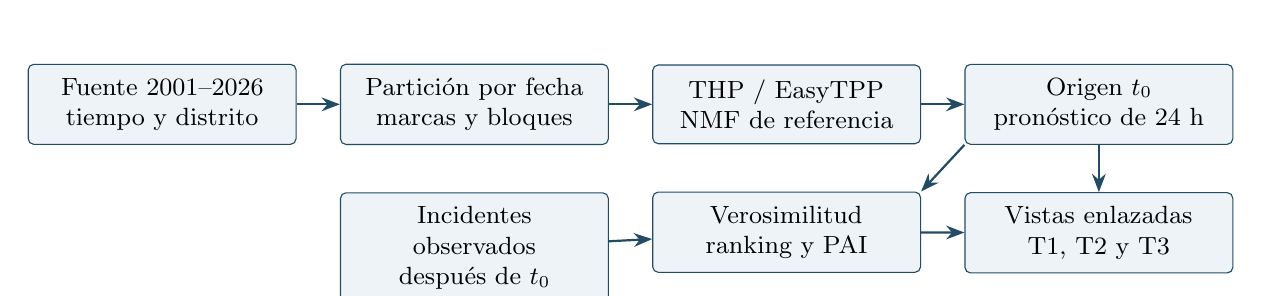
\begin{tikzpicture}[
  font=\small,
  node distance=0.55cm,
  box/.style={draw=azul, rounded corners=2pt, fill=fondo,
    align=center, text width=3.05cm, minimum height=1cm, inner sep=5pt},
  arrow/.style={-{Stealth}, thick, draw=azul}
]
\node[box] (raw) {Fuente 2001--2026\\tiempo y distrito};
\node[box,right=of raw] (split) {Partición por fecha\\marcas y bloques};
\node[box,right=of split] (models) {THP / EasyTPP\\NMF de referencia};
\node[box,right=of models] (predict) {Origen $t_0$\\pronóstico de 24 h};
\node[box,below=0.6cm of predict] (views) {Vistas enlazadas\\T1, T2 y T3};
\node[box,below=0.6cm of split] (future) {Incidentes observados\\después de $t_0$};
\node[box,below=0.6cm of models] (evaluate) {Verosimilitud\\ranking y PAI};
\draw[arrow] (raw)--(split);
\draw[arrow] (split)--(models);
\draw[arrow] (models)--(predict);
\draw[arrow] (predict)--(views);
\draw[arrow] (predict.south west) -- (evaluate.north east);
\draw[arrow] (future)--(evaluate);
\draw[arrow] (evaluate)--(views);
\end{tikzpicture}
\caption{Pipeline propuesto. La rama de incidentes posteriores al origen solo entra en la evaluación; el pronóstico usa el historial anterior y trayectorias simuladas.}
\label{fig:pipeline}
\end{figure*}


\subsection{Datos, territorio y preparación}
La tabla fuente contiene \campo{ID}, \campo{Date}, \campo{Primary Type}, \campo{District}, \campo{Community Area} y otros atributos \cite{chicagoCrimes}. Las salidas del notebook registran 34 tipos de delito y 25 códigos distintos no nulos en \campo{District}, además de 47 distritos faltantes; THEFT (1\,834\,108) y BATTERY (1\,573\,013) son los dos tipos más frecuentes en \emph{toda} la carga. Estos recuentos son descriptivos. La selección definitiva de cinco o seis categorías, la codificación de marcas y cualquier normalización se aprenderán solo del entrenamiento.

La propuesta solicita distritos como unidad espacial. Antes de fijar $|\mathcal D|$, se reconciliarán los 25 códigos históricos presentes en el notebook con el catálogo y los polígonos versionados del sistema policial. La página institucional enumera 22 distritos actuales \cite{cpdDistricts}; por ello, ``23 distritos'' se conserva como hipótesis de diseño y no como recuento verificado del dominio actual. Se documentarán reglas históricas de correspondencia y exclusiones; no se asignará automáticamente un código antiguo a un polígono actual sin evidencia. Con 23 distritos válidos y cinco o seis tipos habría 115--138 marcas; con 22, 110--132. Ambos tamaños son moderados, pero el $M$ definitivo depende de la auditoría territorial. Se guardará el porcentaje de registros cubierto por el dominio elegido.

Se convierten fechas, se valida orden y precisión, se retiran del modelo solo los registros sin tiempo, tipo o distrito válido conforme al catálogo, y se registran exclusiones por motivo. Los \campo{ID} duplicados se inspeccionan; no se borran casos por \campo{Case Number}, ya que los homicidios pueden tener una fila por víctima. El notebook registra abundancia de marcas exactamente a las 00:00; se auditarán empates y posibles horas convencionales antes de asignarles orden arbitrario. Cualquier regla determinista de desempate y su prueba de sensibilidad se documentarán, sin asumir que el orden impuesto represente causalidad. \campo{Arrest}, \campo{Domestic} y \campo{Updated On} no serán variables de entrada del pronosticador. El portal puede revisar registros históricos y \campo{Date} no establece cuándo se conocía cada evento: la evaluación descrita es retrospectiva por fecha del incidente, no una simulación verificada de disponibilidad operativa en tiempo real.

La partición cronológica preliminar usa entrenamiento 2001--2023, validación 2024 y prueba 2025--el último día completo verificable del corte de 2026. No se crean ventanas que crucen los límites de las particiones. El contexto causal anterior puede iniciar un bloque de validación o prueba, pero sus eventos no son etiquetas puntuadas dos veces; los parámetros y la selección de tipos se fijan sin consultar el futuro. Se medirá la cobertura real del último día: el máximo guardado 2026-09-03 00:00:00 no prueba que septiembre de 2026 esté completo.

\subsection{Tres tareas de análisis visual}
Los usuarios previstos son analistas de datos públicos y responsables de planificación que requieren inspeccionar concentraciones y la fiabilidad del pronóstico. Cada tarea se formula como pregunta analítica, independiente de un gráfico particular:

\noindent\tarea{1}: \textbf{Localizar y comparar} los distritos con más incidentes esperados para un tipo de delito o para todos los tipos modelados durante las 24 horas posteriores a un origen seleccionado; distinguir concentraciones estables de cambios entre orígenes.

\noindent\tarea{2}: \textbf{Explorar} la secuencia histórica, el intervalo entre incidentes y la variación temporal de las predicciones en distritos seleccionados, para entender qué contextos observados anteceden a un aumento o descenso pronosticado, sin interpretar la atención como explicación causal.

\noindent\tarea{3}: \textbf{Contrastar} las zonas priorizadas por THP y NMF con los incidentes posteriores retenidos para prueba, para identificar aciertos, omisiones y diferencias por delito, horizonte y presupuesto territorial.

Estas tareas conducen a un mapa distrital para \tarea{1}, una línea de tiempo e historial filtrable para \tarea{2}, y vistas enlazadas de diferencias, observaciones y métricas para \tarea{3}. Selección de distrito, tipo, origen y $K$ coordinarán las vistas. Las observaciones del horizonte se mostrarán solo en modo de evaluación, con una frontera temporal clara entre entrada y resultado.

\subsection{Pipeline y evaluación prevista}
La Fig.~\ref{fig:pipeline} separa explícitamente el entrenamiento, el pronóstico y los datos futuros empleados exclusivamente como verdad de contraste. La implementación partirá del formato de secuencias de EasyTPP, con tiempo desde inicio, intervalo entre eventos y marca codificada \cite{easytppDataset}. Se comprobará por código que los 128 eventos de contexto compartidos no duplican objetivos y que el tramo sin eventos hasta el final de la observación recibe el tratamiento previsto en la log-verosimilitud. Si el adaptador requiere una máscara adicional, se implementará y verificará sobre secuencias pequeñas antes del corpus completo.



Primero se medirán pérdida logarítmica negativa por evento del THP en prueba y exactitud de la siguiente marca conjunta, además de sus componentes delito y distrito y error absoluto o cuadrático del tiempo hasta el siguiente suceso. El protocolo de predicción de siguiente evento y el de mapa multievento usarán únicamente el historial disponible en cada origen: el primero puede condicionarse en el historial real hasta el evento anterior; el segundo debe generar su propio futuro. Se reportarán juntos, pero no se confundirán sus condiciones.

Para la evaluación espacial se fijarán por validación un horizonte principal de 24 h, los valores de $K$, la cantidad de orígenes y una regla estable de desempate. Sea $P_K$ el conjunto de los $K$ distritos pronosticados con mayor puntaje y $O_K$ el de los $K$ distritos con más incidentes observados en el horizonte. Se usará $\operatorname{Precision@}K=|P_K\cap O_K|/K$ como coincidencia de rankings. También se reportará $\operatorname{HitRate@}K=N(P_K)/N(\mathcal D)$, proporción de incidentes futuros capturados; son métricas distintas. Para $A(P_K)$, área de los polígonos predichos, y $A(\mathcal D)$, área total del dominio, $\operatorname{PAI}_K=\operatorname{HitRate@}K/[A(P_K)/A(\mathcal D)]$ \cite{chainey2008utility}. Se excluirán del promedio fechas sin eventos para las que el cociente no esté definido, informando cuántas fueron. Además de $K$ fijo, se compararán métodos con presupuesto de área comparable, ya que los distritos tienen superficies desiguales. El conteo futuro, la definición territorial y las fechas evaluadas serán idénticos para THP y NMF. La incertidumbre de las métricas se estimará por bloques de fechas para respetar dependencia temporal.

La implementación se validará primero de extremo a extremo para THEFT; después se repetirá con las categorías frecuentes de entrenamiento. No se presentan números de verosimilitud, precisión ni PAI hasta entrenar, congelar el protocolo y evaluar el corte de prueba. Las secciones de diseño visual detallado, discusión de resultados y conclusiones corresponderán al proyecto final completo.

\begingroup\small
\bibliographystyle{unsrt}
\bibliography{ref}
\endgroup
\end{document}
